\documentclass[11pt]{article}
\usepackage[margin=1in]{geometry}
\usepackage{amsmath,amssymb}
\usepackage{booktabs,longtable,array,tabularx}
\usepackage{enumitem}
\usepackage{hyperref}
\usepackage{tikz}
\usepackage{tikz-cd}
\usepackage{multicol}
\usepackage{titlesec}

\hypersetup{colorlinks=true,linkcolor=blue,urlcolor=blue,citecolor=blue}
\setlength{\parindent}{0pt}
\setlength{\parskip}{0.75\baselineskip}
\setlist[itemize]{leftmargin=1.5em,itemsep=0.2em}
\setlist[enumerate]{leftmargin=1.5em,itemsep=0.2em}
\renewcommand{\arraystretch}{1.2}
\titleformat{\section}{\Large\bfseries}{Chapter \thesection:}{0.5em}{}
\titleformat{\subsection}{\large\bfseries}{\thesubsection}{0.5em}{}

\title{\textbf{Can Democracy Survive Without an Opposition?}\\[0.5em]
\large Operation Lotus, Party Dominance, and the Future of Indian Democracy}
\author{Bhuvan Raj Guguloth\\Indian Institute of Technology Kharagpur}
\date{\today}

\begin{document}
\maketitle
\thispagestyle{empty}
\newpage

\section*{Declaration}
I hereby declare that the report titled ``Can Democracy Survive Without an Opposition? Operation Lotus, Party Dominance, and the Future of Indian Democracy'' is an original work carried out by me.

This study has been prepared solely for academic and research purposes. The ideas, interpretations, and conclusions presented in this report are based on publicly available information, scholarly literature, constitutional documents, judicial decisions, and political analysis. Wherever the work of other authors and researchers has been used, appropriate acknowledgment and citation has been provided.

I further declare that this report has not been submitted, either wholly or partially, for the award of any degree, diploma, or certification at any institution.

The views expressed in this report are those of the author and do not necessarily reflect the views of any institution, organization, or political entity.

\vspace{2em}
\textbf{Bhuvan Raj Guguloth}\\
Date: \rule{4cm}{0.4pt}\\
Place: \rule{4cm}{0.4pt}
\newpage

\section*{Acknowledgements}
Democracy is not merely a system of government; it is an ongoing conversation between institutions, citizens, and ideas. This report emerged from a desire to better understand that conversation within the context of contemporary Indian politics.

I would like to express my sincere gratitude to the scholars, constitutional thinkers, journalists, policymakers, and public institutions whose work has informed this study. Their contributions to political science, constitutional law, and democratic theory provided the intellectual foundation upon which this report was built.

I owe particular acknowledgment to the works of B. R. Ambedkar, Robert Dahl, Rajni Kothari, Joseph Schumpeter, Steven Levitsky, Daniel Ziblatt, and numerous other scholars whose ideas continue to shape contemporary debates on democracy, federalism, and political competition.

This report also benefited from publicly accessible parliamentary records, judicial decisions, election data, policy reports, and independent journalism that collectively strengthen democratic accountability and public discourse.

Finally, I acknowledge that the study of democracy is itself an exercise in democratic values. The ability to question institutions, examine power, and engage in critical inquiry remains one of the greatest strengths of a constitutional democracy. It is in that spirit of inquiry that this report has been written.

\vspace{2em}
\textbf{Bhuvan Raj Guguloth}\\
Indian Institute of Technology Kharagpur
\newpage

\begin{abstract}
India's parliamentary democracy has historically been characterized by coalition governments, strong regional parties, and competitive multi-party elections. In recent decades, however, political realignments facilitated through defections, resignations, and party splits have become increasingly prominent. Popularly known as ``Operation Lotus,'' these developments have sparked significant debate over democratic legitimacy, federalism, and the balance of political power in India.

This report examines Operation Lotus not merely as a political strategy, but as an institutional phenomenon with broader implications for democratic governance. Through an analysis of major case studies, including Karnataka (2008, 2019), Madhya Pradesh (2020), and Maharashtra (2022), the study investigates how post-election government formation influences electoral mandates, opposition strength, and democratic competition.

The report further situates Operation Lotus within broader theories of democratic backsliding and dominant-party systems. It explores whether repeated political consolidation can gradually weaken coalition politics, reduce the influence of regional parties, and contribute to the centralization of political power while retaining formal democratic procedures. Special attention is given to debates surrounding double-engine governments, delimitation, and the proposed One Nation, One Election framework.

The study argues that democracy cannot be evaluated solely through the existence of elections. Rather, its health depends equally on meaningful political competition, institutional autonomy, federal balance, and the continued viability of opposition parties. While Operation Lotus often operates within constitutional boundaries, its repeated use raises important questions about whether constitutional legality necessarily guarantees democratic legitimacy.
\end{abstract}
\newpage
\tableofcontents
\newpage

\section{Introduction}
India is often celebrated as the world's largest democracy. Since independence in 1947, the country has sustained universal adult suffrage, regular elections, and peaceful transfers of power across multiple political parties. The Indian democratic experience is particularly remarkable given its immense social, linguistic, religious, and regional diversity.

However, democracy is not merely the conduct of elections. Modern democratic theory suggests that the health of a democracy depends not only on electoral participation but also on meaningful political competition, institutional autonomy, federal balance, and an effective opposition.

In recent years, Indian politics has witnessed an increasing number of instances in which governments have changed not through elections but through defections, resignations, and party realignments. These political developments, popularly referred to as ``Operation Lotus,'' have emerged as one of the most debated phenomena in contemporary Indian democracy.

Supporters argue that such practices are legitimate features of parliamentary systems, where governments derive authority from legislative majorities rather than direct popular election. Critics contend that repeated political defections may undermine electoral mandates, weaken opposition parties, and contribute to the concentration of political power.

The debate surrounding Operation Lotus extends beyond questions of party politics. It raises broader concerns regarding democratic legitimacy, constitutional morality, and the future of India's federal structure. At the heart of this study lies a fundamental question: \emph{Can democracy remain healthy if elections continue, but meaningful political competition gradually declines?}

\subsection{Background and Historical Context}
The evolution of Indian democracy since independence can broadly be divided into three political phases: the Congress-dominant era (1947--1989), the coalition era (1989--2014), and the contemporary period characterized by the rise of the Bharatiya Janata Party (BJP) as a dominant national political force.

\textbf{The Congress System (1947--1989).} Following independence, the Indian National Congress emerged as the dominant political party. Political scientist Rajni Kothari described this period as the ``Congress System,'' in which the Congress functioned not merely as a political party but also as a broad umbrella accommodating diverse ideological factions. Although opposition parties existed, Congress exercised overwhelming influence at both national and state levels for several decades. The Emergency (1975--1977) remains a critical reminder of the risks associated with excessive concentration of political power, while the peaceful electoral defeat of Congress in 1977 demonstrated democratic resilience.

\textbf{The Coalition Era (1989--2014).} The 1989 general election marked a major turning point. Coalition governments became the norm rather than the exception, and regional parties such as DMK, AIADMK, TDP, SP, BSP, JD(U), Shiv Sena, and Trinamool Congress became important actors in national governance.

\begin{longtable}{llllr}
\caption{Major Coalition Governments in India (1989--2014)}\\
\toprule
Period & Prime Minister & Coalition & Largest Party & Seats\\
\midrule
\endfirsthead
\toprule
Period & Prime Minister & Coalition & Largest Party & Seats\\
\midrule
\endhead
1989--1990 & V. P. Singh & National Front & Janata Dal & 143\\
1991--1996 & P. V. Narasimha Rao & Minority Congress Govt. & INC & 232\\
1996--1998 & Deve Gowda / Gujral & United Front & Janata Dal & 46\\
1998--1999 & A. B. Vajpayee & NDA-I & BJP & 182\\
1999--2004 & A. B. Vajpayee & NDA-II & BJP & 182\\
2004--2009 & Manmohan Singh & UPA-I & INC & 145\\
2009--2014 & Manmohan Singh & UPA-II & INC & 206\\
\bottomrule
\end{longtable}

\begin{table}[h]
\centering
\caption{Coalition Composition of UPA-I (2004)}
\begin{tabular}{lr}
\toprule
Party & Seats\\
\midrule
INC & 145\\
RJD & 24\\
DMK & 16\\
NCP & 9\\
PMK & 6\\
LJP & 4\\
Left Front (External Support) & 61\\
\bottomrule
\end{tabular}
\end{table}

\textbf{The Return of Majority Governments.} The 2014 general election marked another significant turning point. For the first time in nearly three decades, a single party secured an outright majority in the Lok Sabha.

\begin{table}[h]
\centering
\caption{Largest Party in Lok Sabha Elections}
\begin{tabular}{llrl}
\toprule
Election Year & Largest Party & Seats Won & Majority Achieved?\\
\midrule
2004 & INC & 145 & No\\
2009 & INC & 206 & No\\
2014 & BJP & 282 & Yes\\
2019 & BJP & 303 & Yes\\
2024 & BJP & 240 & No (NDA Majority)\\
\bottomrule
\end{tabular}
\end{table}

Unlike previous coalition governments, the BJP in 2014 possessed an independent majority without relying on alliance partners for government formation. This marked a structural shift from dependence on coalitions toward majority governance. It also coincided with the increasing prominence of the ``double-engine government'' narrative, which argues that governance becomes more efficient when the same party governs both the Centre and the state.

\subsection{Problem Statement}
The phenomenon popularly referred to as Operation Lotus has emerged as one of the most debated developments in contemporary Indian politics. Through defections, resignations, and political realignments, governments in several states have changed without fresh electoral mandates. While such transitions often occur within constitutional frameworks, they raise questions regarding democratic legitimacy and institutional balance.

Parliamentary democracies derive governments from legislative majorities rather than direct executive elections. Consequently, governments may legitimately lose or gain majority support between elections. However, repeated instances of post-election government formation through defections create a tension between two democratic principles: legislative flexibility and electoral mandate.

The central challenge of this report is therefore not to determine whether Operation Lotus is legal, but to investigate a deeper constitutional and democratic question: \emph{Can a practice be constitutionally valid while simultaneously weakening substantive democracy?}

\subsection{Research Questions and Hypothesis}
The primary objective of this report is to examine whether Operation Lotus represents a routine feature of parliamentary democracy or whether its repeated use contributes to democratic backsliding and dominant-party consolidation in India.

\textbf{Primary Research Question:} Does Operation Lotus contribute to democratic backsliding in India?

\textbf{Secondary Research Questions:}
\begin{enumerate}
\item How do political defections affect electoral mandates and voter representation?
\item Does the repeated use of post-election realignments weaken opposition parties and political competition?
\item What role do institutions such as the Speaker, Governor, and Judiciary play during political transitions?
\item Is India transitioning from a multi-party federal democracy toward a dominant-party system?
\item How might delimitation and One Nation, One Election influence democratic competition in a dominant-party environment?
\end{enumerate}

\textbf{Hypothesis:} While Operation Lotus may operate within constitutional frameworks, its repeated use contributes to democratic centralization by weakening opposition parties, reducing coalition constraints, and facilitating dominant-party politics.

\textbf{Null Hypothesis:} Operation Lotus represents a legitimate mechanism of parliamentary democracy and does not significantly affect democratic competition or institutional balance.

The study focuses on political developments in India from 2008 to 2024, with emphasis on Karnataka, Madhya Pradesh, Maharashtra, Goa, Manipur, Arunachal Pradesh, anti-defection law, double-engine governments, delimitation, One Nation One Election, federalism, and regional parties.

\section{Literature Review}
The debate surrounding Operation Lotus intersects with multiple strands of political science literature, including democratic backsliding, dominant-party systems, parliamentary democracy, and federalism. While the term itself is politically contested, the broader phenomena it represents---political defections, government instability, and concentration of power---have long been subjects of academic inquiry.

\subsection{Democratic Backsliding}
Traditional understandings of democratic decline often focused on military coups and abrupt regime changes. Contemporary scholars argue that democracies increasingly erode through gradual institutional weakening rather than sudden collapse. Levitsky and Ziblatt argue that modern democracies frequently deteriorate from within through elected leaders who weaken institutional constraints, reduce political competition, and undermine democratic norms while preserving formal electoral procedures. Bermeo similarly describes democratic backsliding as processes through which democratic institutions weaken incrementally while maintaining constitutional appearances.

These frameworks suggest that elections alone are insufficient for evaluating democratic health. This literature is relevant to India, where elections continue to remain competitive, yet debates have emerged regarding institutional autonomy, opposition strength, and political centralization.

\subsection{Dominant-Party Systems}
Political scientists distinguish between one-party states and dominant-party democracies. A one-party state legally prohibits competition, whereas a dominant-party system allows elections but features prolonged rule by a single political party. Dominant-party systems have existed in Japan under the Liberal Democratic Party, South Africa under the African National Congress, Mexico under the Institutional Revolutionary Party, and India under the Congress System.

These cases demonstrate that democracies may retain electoral institutions while political competition becomes increasingly unequal. They raise the question of whether the rise of the BJP indicates a new dominant-party system in India.

\subsection{Parliamentary Democracy and Political Defections}
Parliamentary systems derive executive authority from legislative majorities. Governments may legitimately change between elections if they lose majority support in the legislature. Political defections and coalition realignments are therefore not inherently undemocratic. However, excessive party switching can weaken accountability and voter trust. India's Tenth Schedule, introduced through the 52nd Constitutional Amendment in 1985, sought to curb opportunistic defections. Critics argue that mass resignations and party splits have created pathways around anti-defection provisions.

\subsection{Federalism and Regional Parties}
India's federal structure has historically been strengthened by regional parties. During the coalition era, regional actors became indispensable to national governments. Their decline may have implications beyond electoral outcomes, potentially affecting federal bargaining, policy diversity, and political pluralism.

\subsection{Research Gap}
Substantial scholarship exists on democratic backsliding, party systems, and federalism, but relatively limited academic work examines Operation Lotus as a case study of democratic transformation in contemporary India. This study bridges that gap by integrating constitutional law, electoral data, and comparative political theory.

\section{Theoretical Framework}
\subsection{What is Democracy?}
Democracy is often understood as a system in which governments are elected by the people through free and fair elections. Yet contemporary political science treats democracy as a multidimensional concept. Robert Dahl's concept of polyarchy emphasizes not only elections but also participation, competition, and civil liberties.

Modern democracies are evaluated across several dimensions: free and fair elections, political competition, civil liberties, institutional independence, rule of law, and accountability. Democracy is therefore not merely a mechanism for choosing governments but also a framework for limiting power and ensuring representation.

\textbf{Procedural democracy} focuses on regular elections, universal suffrage, majority rule, and constitutional governance. From this perspective, governments formed through legislative majorities remain valid if political alignments change after elections.

\textbf{Substantive democracy} asks whether democratic values are meaningfully realized: whether citizens possess real choices, opposition parties can compete fairly, institutions remain independent, and power remains accountable.

Joseph Schumpeter viewed democracy as competition for political leadership. Under this view, democracy requires multiple political alternatives, uncertainty of outcomes, and the realistic possibility of governments losing power. A healthy democracy is measured not only by the strength of its government, but also by the viability of its opposition.

\subsection{Democratic Backsliding}
The decline of democracies in the twenty-first century differs from older forms of breakdown. Contemporary democracies often erode gradually while retaining elections, courts, legislatures, and opposition parties. Indicators include weakening of opposition, concentration of power, institutional capture, declining federal balance, and unequal electoral competition.

This report evaluates democratic health using five dimensions.

\begin{table}[h]
\centering
\caption{Analytical Framework for Democratic Health}
\begin{tabularx}{\textwidth}{lX}
\toprule
Dimension & Key Question\\
\midrule
Electoral Competition & Are elections meaningfully competitive?\\
Opposition Strength & Can opposition parties effectively challenge incumbents?\\
Institutional Independence & Are institutions autonomous and impartial?\\
Federalism & Do states retain meaningful autonomy?\\
Political Pluralism & Do citizens possess genuine political alternatives?\\
\bottomrule
\end{tabularx}
\end{table}

\subsection{Dominant-Party Systems and Political Competition}
A dominant-party system differs from a one-party state because opposition parties are legally permitted and elections continue. However, one party consistently maintains political dominance over an extended period.

\begin{table}[h]
\centering
\caption{One-Party State vs Dominant-Party Democracy}
\begin{tabular}{lll}
\toprule
Characteristic & One-Party State & Dominant-Party Democracy\\
\midrule
Opposition Parties & Not permitted & Permitted\\
Elections & Limited or absent & Regular elections\\
Political Competition & Restricted & Present but unequal\\
Examples & China & Japan, South Africa, Mexico\\
\bottomrule
\end{tabular}
\end{table}

Dominant-party systems may emerge due to charismatic leadership, strong organization, fragmented opposition, electoral advantages, national narratives, and institutional incumbency. Dominance does not necessarily imply democratic decline, but extended dominance may reduce accountability and weaken institutional checks. The key question is whether meaningful competition remains possible.

\subsection{Constitutional Morality, Legality, and Democratic Legitimacy}
A government may satisfy constitutional procedure while raising concerns about democratic ethics, representation, and institutional norms. Constitutional legality asks whether an action is permitted under the Constitution and law. Democratic legitimacy asks whether power reflects the spirit of democratic representation.

Citizens often vote for parties, alliances, ideologies, and leaders as well as individual candidates. When governments change through post-election defections rather than fresh elections, questions arise regarding voter intent.

B. R. Ambedkar emphasized that constitutional governance requires adherence not only to the letter of law but to its underlying democratic spirit. ``Constitutional morality is not a natural sentiment. It has to be cultivated.'' Operation Lotus sits at the intersection of constitutional legality and democratic legitimacy.

\subsection{Federalism, Opposition, and Democratic Pluralism}
India's federal system distributes power across the Union, states, and local governments. Federalism is not merely administrative; it is a democratic safeguard against concentration of power. Regional parties represent local interests, strengthen federalism, act as checks on central authority, and increase policy diversity.

Opposition parties scrutinize executive action, hold governments accountable, provide alternative policy visions, and represent minority viewpoints. Democracy thrives not in uniformity, but in the coexistence of competing voices and institutions.

\section{Understanding Operation Lotus}
\subsection{Origin and Evolution of the Term}
The term ``Operation Lotus'' derives from the lotus, the electoral symbol of the BJP, and is commonly used by political observers and media to describe strategies through which legislative majorities are altered outside direct electoral outcomes. The broader phenomenon of political defections is neither new nor unique to any single party, but the scale, frequency, and strategic use of defections in recent years have renewed debate.

\subsection{Political Defections in Historical Context}
Political defections have a long history in India. The phrase ``Aya Ram, Gaya Ram'' entered political vocabulary in 1967 after Haryana legislator Gaya Lal changed parties multiple times within a short period. Concerns over instability, corruption, weak party discipline, and erosion of trust eventually led to anti-defection reforms.

\subsection{The Anti-Defection Law}
The 52nd Constitutional Amendment introduced the Tenth Schedule in 1985. It disqualifies legislators who voluntarily give up party membership, vote against party directions, or defy party leadership in crucial legislative matters. The Speaker decides disqualification cases.

\begin{table}[h]
\centering
\caption{Objectives and Challenges of the Anti-Defection Law}
\begin{tabularx}{\textwidth}{lll}
\toprule
Objective & Intended Outcome & Criticism\\
\midrule
Prevent defections & Political stability & Limits legislator autonomy\\
Enforce party discipline & Stable governments & Strengthens party leadership\\
Reduce corruption & Greater accountability & Speaker may act politically\\
\bottomrule
\end{tabularx}
\end{table}

\subsection{How Operation Lotus Functions}
Although political events differ across states, Operation Lotus is often described as following a recurring pattern: a hung assembly or fragile coalition emerges; legislators resign, shift allegiance, or coalition partners withdraw support; the incumbent loses majority; and a new government is formed through revised legislative arithmetic.

\begin{figure}[h]
\centering
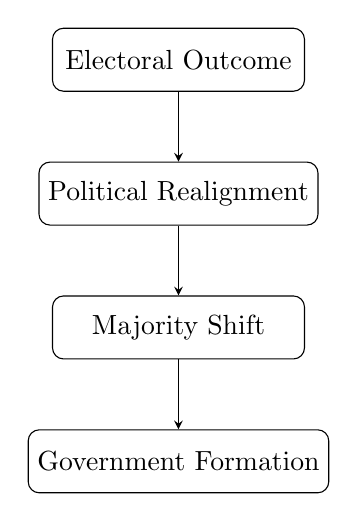
\begin{tikzpicture}[node distance=1.7cm,>=stealth,every node/.style={draw,rounded corners,align=center,minimum width=3.2cm,minimum height=0.8cm}]
\node (a) {Electoral Outcome};
\node (b) [below of=a] {Political Realignment};
\node (c) [below of=b] {Majority Shift};
\node (d) [below of=c] {Government Formation};
\draw[->] (a) -- (b);
\draw[->] (b) -- (c);
\draw[->] (c) -- (d);
\end{tikzpicture}
\caption{Operation Lotus Mechanism}
\end{figure}

Mechanisms include defections, resignations, party splits, and coalition withdrawal. Operation Lotus may simultaneously be a constitutionally permissible strategy, a politically effective mechanism, and a democratically contested practice.

\section{Case Studies of Operation Lotus}
\subsection{Introduction}
Operation Lotus has evolved from a state-level political strategy into a broader phenomenon shaping contemporary Indian politics. Cases may be classified as successful, attempted, or contested.

\begin{longtable}{@{}p{0.17\textwidth}p{0.11\textwidth}p{0.21\textwidth}p{0.21\textwidth}p{0.14\textwidth}@{}}
\caption{Classification of Operation Lotus Cases (2008--2026)}\\
\toprule
State/Institution & Year & Mechanism & Outcome & Classification\\
\midrule
\endfirsthead
\toprule
State/Institution & Year & Mechanism & Outcome & Classification\\
\midrule
\endhead
Karnataka & 2008 & Defections/support & Government changed & Successful\\
Karnataka & 2019 & Resignations & Government changed & Successful\\
Madhya Pradesh & 2020 & Resignations & Government changed & Successful\\
Maharashtra & 2022 & Party split & Government changed & Successful\\
Goa & 2019, 2022 & Defections & Government strengthened/changed & Successful\\
Arunachal Pradesh & 2016 & Party merger & Government changed & Successful\\
Manipur & Multiple & Coalition shifts & Government changed & Contested\\
Bihar & 2024--2026 & Alliance realignment & Government changed & Contested\\
West Bengal & 2021--2026 & Defections/expansion & Government unchanged & Attempted\\
Delhi & 2022 onward & Alleged MLA poaching & Government unchanged & Attempted\\
Punjab/AAP & 2026 & Rajya Sabha defections & Parliamentary shift & Successful\\
\bottomrule
\end{longtable}

\subsection{Karnataka (2008): The Birth of Operation Lotus}
The 2008 Karnataka Assembly election produced a fragmented verdict: BJP won 110 seats, INC 80, JD(S) 28, and others 6, with a majority mark of 113. Support from independents and subsequent realignments enabled the BJP to secure power. The term ``Operation Kamala'' or ``Operation Lotus'' gained prominence during this period.

\subsection{Karnataka (2019): Collapse of Coalition Government}
The Congress--JD(S) coalition formed government despite the BJP emerging as the largest party. Resignations by multiple MLAs reduced the effective strength of the Assembly, and the coalition lost majority. The case raised questions about whether mass resignations circumvent the spirit of anti-defection laws.

\subsection{Madhya Pradesh (2020): Leadership Defection and Government Change}
The resignation of Jyotiraditya Scindia from the Congress and the subsequent resignation of supporting MLAs led to the fall of the Kamal Nath government. The BJP returned to power under Shivraj Singh Chouhan. The case highlights whether leadership defections differ from individual defections and whether anti-defection law adequately addresses coordinated resignations.

\subsection{Maharashtra (2022): Party Identity and Legislative Majority}
The split within Shiv Sena under Eknath Shinde triggered a major constitutional crisis. It raised questions regarding party identity, whip legitimacy, legislative majority, and judicial review. The democratic question was: who owns a political party---its organization or its legislators?

\subsection{Goa, Arunachal Pradesh, Manipur, Bihar, West Bengal, Delhi, and Punjab}
Small assemblies such as Goa and Arunachal Pradesh can be especially susceptible to political realignments. Manipur illustrates how regional dynamics and coalition arithmetic shape governance in smaller states. Bihar presents a complex case of alliance switching by party leadership rather than direct defections. West Bengal is a counterexample where strong regional identity limited political consolidation. Delhi and Punjab involve alleged poaching attempts, while recent parliamentary defections expanded the debate beyond state legislatures.

\subsection{Comparative Findings}
The cases reveal several patterns: coalition governments are more vulnerable to realignment; institutional actors play decisive roles; the anti-defection law contains exploitable loopholes; and regional parties remain important democratic counterweights. Operation Lotus is not a singular event but an evolving political strategy whose democratic implications depend on cumulative impact.

\section{Institutions Under Stress}
\subsection{Introduction}
Democracies are sustained not only through elections but also through institutions that regulate political competition. Political realignments are shaped by the Anti-Defection Law, the Speaker, the Governor, and the Judiciary. The repeated occurrence of defections and government changes raises the question of whether institutions are adequately equipped to preserve democratic legitimacy.

\subsection{The Anti-Defection Law}
The anti-defection law seeks to promote stability, discourage opportunistic defections, protect mandates, and strengthen party discipline. Yet contemporary developments have exposed limitations.

\begin{table}[h]
\centering
\caption{Strengths and Weaknesses of the Anti-Defection Law}
\begin{tabularx}{\textwidth}{XX}
\toprule
Strengths & Weaknesses\\
\midrule
Prevents individual defections & Encourages mass defections\\
Promotes stable governments & Limits legislator autonomy\\
Reduces political instability & Concentrates power in party leadership\\
Protects party systems & Vulnerable to strategic resignations\\
\bottomrule
\end{tabularx}
\end{table}

Recent events suggest that while the law reduced individual defections, it may have incentivized collective resignations and party splits.

\subsection{The Speaker, Governor, and Judiciary}
Under the Tenth Schedule, the Speaker decides disqualification petitions. Because Speakers are usually party members, concerns arise regarding neutrality, delays, timing, and recognition of factions. The Governor's office has powers related to government formation, floor tests, and President's Rule, but discretionary powers have often generated controversy. The judiciary acts as constitutional interpreter in disputes involving floor tests, disqualification, party splits, and government formation, but delays and enforcement challenges remain concerns.

\subsection{Institutional Incentives and Democratic Outcomes}
Political outcomes are not determined solely by party strategies. They are shaped by institutional incentives embedded within constitutional structures. Operation Lotus may therefore be understood not merely as a political strategy but also as a product of institutional design.

\section{Electoral Mandate vs Legislative Majority}
At the heart of the debate lies a fundamental question: who owns the electoral mandate? In parliamentary democracies, governments derive authority from legislative majorities. Yet elections are fought by parties, alliances, and leaders. This creates a tension between legislative autonomy and electoral representation.

\subsection{Individuals, Parties, and Voters}
The Indian electoral system formally elects individual legislators, but voting behavior is often shaped by party ideology, leadership, alliances, local candidates, and national narratives. If voters choose candidates because of party affiliation, changing parties after elections may alter the original mandate.

Supporters of legislative autonomy argue that representatives should act according to conscience, constituency interests, and changing political circumstances. Critics argue that elections increasingly revolve around parties and leaders, and defections may distort voter expectations.

\subsection{Coalition Governments and Mandates}
Coalitions complicate representation. Voters may support individual candidates, parties, pre-poll alliances, or post-poll coalitions. Cases from Bihar, Maharashtra, and Karnataka demonstrate how coalition politics blurs mandates. The debate ultimately concerns the meaning of democratic representation: democracy requires not only the right to elect governments, but confidence that electoral choices will be respected.

\section{Beyond Operation Lotus: Political Consolidation and the Future of Indian Democracy}
Operation Lotus should also be understood within broader processes of political consolidation. Political expansion through elections is a normal feature of democracy. The question is whether cumulative effects alter the quality of democratic competition.

\subsection{Operation Lotus 1.0 and 2.0}
Operation Lotus 1.0 focuses on legislative majorities, government formation, defections, and resignations. Examples include Karnataka, Madhya Pradesh, and Maharashtra. Operation Lotus 2.0, as an analytical category, focuses on electoral expansion, institutional consolidation, opposition fragmentation, narrative dominance, Rajya Sabha realignments, and strategic alliances.

\subsection{Double-Engine Governments}
The double-engine government narrative suggests governance becomes more efficient when the same party governs both Union and State. Supporters emphasize coordination, faster implementation, administrative efficiency, and reduced conflict. Critics worry that regional parties may face structural disadvantages and federal bargaining may weaken.

\subsection{One Nation, One Election and Delimitation}
One Nation, One Election seeks to synchronize national and state elections. Supporters point to lower costs, governance continuity, and reduced administrative burden. Critics argue that national issues may overshadow state concerns and benefit nationally dominant parties.

Delimitation determines allocation of Lok Sabha seats and electoral boundaries. States with higher population growth may gain representation, while states that controlled population growth may experience relative decline. This has implications for federal balance, regional representation, and political competition.

\subsection{Dominant-Party Democracy and Democratic Resilience}
Dominant-party systems can produce policy continuity, stability, and long-term planning, but also risks of weakened opposition, centralization, reduced accountability, and institutional capture. India's democratic future depends not on the success or failure of one party, but on whether institutions preserve meaningful competition.

\section{Comparative Perspectives: Dominant-Party Systems Across Democracies}
\subsection{Japan: Liberal Democratic Party}
Japan's LDP governed almost continuously from 1955 with brief interruptions. Its dominance was supported by strong organization, economic growth, fragmented opposition, and stable leadership. Yet Japan retained competitive elections, independent institutions, and peaceful transfers of power. This shows that dominance does not inevitably become authoritarian, though it can weaken opposition capacity.

\subsection{Mexico: Institutional Revolutionary Party}
Mexico's PRI governed for roughly seventy-one years. Elections continued, but critics argued that patronage, institutional influence, and incumbency advantages reduced equality of competition. The PRI's eventual defeat in 2000 shows that even long-standing dominant-party systems can experience democratic transition.

\subsection{South Africa: African National Congress}
Since 1994 the ANC has been South Africa's dominant party, rooted in anti-apartheid legitimacy and broad coalitions. Over time, concerns emerged regarding accountability, corruption, and reduced competition. Recent elections demonstrate that dominance can decline when institutions and civil society remain active.

\subsection{India's Congress System}
India previously experienced one-party predominance under the Congress. The Emergency illustrated the risks of concentrated power, while the 1977 defeat showed democratic resilience.

\begin{table}[h]
\centering
\caption{Comparing India's Two Dominant-Party Eras}
\begin{tabularx}{\textwidth}{lXX}
\toprule
Feature & Congress Era & BJP Era\\
\midrule
Dominant Party & INC & BJP\\
Period & 1947--1989 & 2014--present\\
Political Context & Post-independence nation-building & Liberalized economy and digital politics\\
Opposition Strength & Weak but emerging & Fragmented but active\\
Federal Structure & Centralized & Strong state variation\\
\bottomrule
\end{tabularx}
\end{table}

\subsection{Comparative Lessons}
Dominance is not necessarily authoritarian; institutions matter; opposition is essential; and dominance can be reversed. The ultimate test of democracy is not whether governments win elections, but whether they can lose them.

\section{Democratic Safeguards and Policy Recommendations}
\subsection{Reforming the Anti-Defection Law}
The anti-defection law may require reform to address coordinated resignations and large-scale defections. Policy options include mandatory re-election for legislators who resign and join another party, cooling-off periods before defectors can hold ministerial office, and narrowing exceptions regarding mergers and splits.

\subsection{Independent Adjudication of Defection Cases}
Disqualification decisions could be transferred from the Speaker to a more independent body, such as the Election Commission or a constitutional tribunal. The objective should be impartial adjudication rather than elimination of political competition.

\subsection{Reforming the Governor's Office}
Reforms could include time-bound floor tests, clearer constitutional guidelines, greater transparency, and codification of conventions. Such measures may reduce uncertainty during government formation.

\subsection{Strengthening Federalism and Electoral Accountability}
Federalism may be strengthened through greater consultation with states, stronger intergovernmental institutions, protection of fiscal federalism, and enhanced state autonomy in designated domains. Electoral reforms may include campaign finance transparency, internal party democracy, and stronger parliamentary deliberation.

\subsection{Safeguarding Institutional Independence}
Public confidence in the judiciary, Election Commission, investigative agencies, and constitutional offices is essential. Institutional independence does not mean freedom from criticism; it means the capacity to act impartially according to constitutional principles.

\section{Conclusion}
This report began with a central question: can democracy remain healthy when political competition becomes increasingly unequal? The analysis examined Operation Lotus through democratic theory, constitutional law, federalism, institutional design, and comparative politics.

Operation Lotus is not a singular event. It represents a broader set of strategies involving defections, resignations, party splits, coalition realignments, and parliamentary shifts. These strategies may operate within constitutional frameworks while producing consequences beyond immediate government formation.

Constitutional legality and democratic legitimacy are not always identical. Governments formed through legislative majorities may satisfy legal requirements, but legitimacy also depends on voter expectations, electoral mandates, fair competition, and institutional trust.

Institutions play a decisive role. The Anti-Defection Law, Speaker, Governor, and Judiciary significantly influence political crises. Regional parties continue to act as democratic counterweights, and India's federal diversity remains a source of resilience.

This report does not conclude that India has ceased to be a democracy. India continues to possess competitive elections, peaceful transfers of power, judicial review, federal institutions, and active political participation. Yet democracy cannot be measured solely by the existence of elections. It also requires meaningful opposition, institutional autonomy, political pluralism, and genuine electoral competition.

The Indian experience reinforces an important insight: democracy is not merely the right to elect governments; it is also the ability to meaningfully replace them. The ultimate strength of democracy is not measured by how effectively governments win power, but by how fairly power can be contested, transferred, and constrained.

\newpage
\section*{List of Tables}
\addcontentsline{toc}{section}{List of Tables}
Table 1: Major Coalition Governments in India (1989--2014)\\
Table 2: Coalition Composition of UPA-I (2004)\\
Table 3: Largest Party in Lok Sabha Elections\\
Table 4: Analytical Framework for Democratic Health\\
Table 5: One-Party State vs Dominant-Party Democracy\\
Table 6: Objectives and Challenges of the Anti-Defection Law\\
Table 7: Classification of Operation Lotus Cases (2008--2026)\\
Table 8: Strengths and Weaknesses of the Anti-Defection Law\\
Table 9: Comparing India's Two Dominant-Party Eras

\section*{List of Figures}
\addcontentsline{toc}{section}{List of Figures}
Figure 1: Operation Lotus Mechanism

\section*{Abbreviations}
\addcontentsline{toc}{section}{Abbreviations}
\begin{longtable}{ll}
\toprule
Abbreviation & Full Form\\
\midrule
BJP & Bharatiya Janata Party\\
INC & Indian National Congress\\
NDA & National Democratic Alliance\\
UPA & United Progressive Alliance\\
AAP & Aam Aadmi Party\\
TMC & Trinamool Congress\\
BJD & Biju Janata Dal\\
JD(U) & Janata Dal (United)\\
RJD & Rashtriya Janata Dal\\
DMK & Dravida Munnetra Kazhagam\\
AIADMK & All India Anna Dravida Munnetra Kazhagam\\
TDP & Telugu Desam Party\\
ONOE & One Nation, One Election\\
LDP & Liberal Democratic Party\\
PRI & Institutional Revolutionary Party\\
ANC & African National Congress\\
\bottomrule
\end{longtable}

\section*{Bibliography}
\addcontentsline{toc}{section}{Bibliography}
\subsection*{Books}
Dahl, R. A. (1971). \emph{Polyarchy: Participation and Opposition}. Yale University Press.\\
Levitsky, S., \& Ziblatt, D. (2018). \emph{How Democracies Die}. Crown.\\
Kothari, R. (1964). The Congress System in India.\\
Schumpeter, J. A. (1942). \emph{Capitalism, Socialism and Democracy}.\\
Pempel, T. J. (1990). \emph{Uncommon Democracies}.\\
Austin, G. (1999). \emph{Working a Democratic Constitution}.

\subsection*{Journal Articles}
Bermeo, N. (2016). On Democratic Backsliding. \emph{Journal of Democracy}.\\
Stepan, A. (1999). Federalism and Democracy. \emph{Journal of Democracy}.\\
Tushnet, M. (2004). Constitutional Hardball. \emph{Georgetown Law Journal}.

\newpage
\appendix
\section{Timeline of Operation Lotus Cases (2008--2026)}
This appendix provides a chronological overview of major political events in India that have been associated with, or discussed in relation to, Operation Lotus. The classification is analytical and does not imply judicial or constitutional determination.

\begin{longtable}{@{}p{0.08\textwidth}p{0.14\textwidth}p{0.15\textwidth}p{0.23\textwidth}p{0.14\textwidth}p{0.11\textwidth}@{}}
\caption{Chronology of Major Operation Lotus Cases}\\
\toprule
Year & State/Institution & Government Before & Political Development & Mechanism & Classification\\
\midrule
\endfirsthead
\toprule
Year & State/Institution & Government Before & Political Development & Mechanism & Classification\\
\midrule
\endhead
2008 & Karnataka & Hung Assembly & BJP secured support and defections & Defections/support & Successful\\
2016 & Arunachal Pradesh & Congress & Large-scale shifts and mergers & Party merger & Successful\\
2017 & Goa & Congress largest party & BJP formed government through alliances & Coalition formation & Contested\\
2017 & Manipur & Hung Assembly & BJP formed government despite not being largest & Coalition building & Contested\\
2019 & Karnataka & INC--JD(S) & MLA resignations led to fall of government & Resignations & Successful\\
2019 & Goa & Congress weakened & Congress MLAs joined BJP & Defections & Successful\\
2020 & Madhya Pradesh & Congress & Scindia and supporting MLAs resigned & Resignations & Successful\\
2021 & West Bengal & TMC & High-profile defections before elections & Defections & Attempted\\
2022 & Maharashtra & MVA & Shiv Sena split under Eknath Shinde & Party split & Successful\\
2022 & Goa & Congress opposition & Multiple MLAs defected to BJP & Defections & Successful\\
2022 & Delhi & AAP & Allegations of MLA poaching & Alleged defections & Attempted\\
2022 & Punjab & AAP & Allegations of inducements & Alleged defections & Attempted\\
2023--2025 & Manipur & BJP-led coalition & Instability and coalition shifts & Realignment & Contested\\
2024 & Bihar & Grand Alliance & Nitish Kumar rejoined NDA & Alliance realignment & Contested\\
2025 & Bihar & NDA & NDA secured decisive electoral victory & Electoral consolidation & Not Operation Lotus\\
2026 & Rajya Sabha & AAP representation & AAP MPs defected to BJP & Parliamentary defections & Successful\\
2026 & West Bengal & TMC & Continued defections and contestation & Political expansion & Attempted\\
\bottomrule
\end{longtable}

\textbf{Classification Framework.} Successful cases are those where political realignment directly altered government formation or legislative balance. Attempted cases involve political expansion, defections, or alleged inducements that did not alter government formation. Contested cases are those where scholars and political actors disagree on whether the events constitute Operation Lotus.

\textbf{Key Observations.} Coalition governments appear more vulnerable to political realignment than majority governments. The anti-defection law has reduced individual defections but may have encouraged collective resignations and party splits. Regional parties continue to act as important democratic counterweights in states such as West Bengal, Tamil Nadu, and Punjab. The phenomenon reflects not only party strategy but also institutional incentives embedded within India's parliamentary system.

\section{Lok Sabha Election Results (1989--2024)}
This appendix may be expanded with constituency-level or party-level data for each Lok Sabha election between 1989 and 2024.

\section{Major Supreme Court Judgments}
\begin{itemize}
\item \emph{Kihoto Hollohan v. Zachillhu} (1992)
\item \emph{Nabam Rebia v. Deputy Speaker} (2016)
\item \emph{Shiv Sena v. Speaker} (2023)
\end{itemize}

\section{Relevant Constitutional Provisions}
\begin{itemize}
\item Tenth Schedule: Anti-defection provisions
\item Article 356: President's Rule
\item Articles concerning the Governor's constitutional role
\end{itemize}

\end{document}
